\section{Desarrollo}
\subsection{Ejercicios}
\label{sec:desar}
\textbf{Ejercicio 1.}

Del diagrama de la figura \ref{fig:esquemas}:

\begin{equation}
X_i = Y_{i-1}\cdot G_{i}\\
Y_{i-1} = h \cdot X_{i-1} + W_{i-1}
\end{equation}

\begin{equation}
\hspace{-4.3cm} [Y_{i-1}] = VAR [h \cdot X_{i-1} + W_{i-1}]
\end{equation}
\begin{equation*}
\hspace{2cm} = h^2 \cdot VAR [X_{i-1}] + 2COV[X_{i-1}, W_{i-1}] + VAR [W_{i-1}]
\end{equation*}

Por ser $X$ y $W$ independientes $COV[X_{i-1}, W_{i-1}] = 0$ . Queda entonces:

\begin{equation}
VAR[Y_{i-1}] = h^2 \cdot A^2 + \sigma_w^2
\end{equation}
\begin{equation}
VAR [X_i] = VAR [G_{i} \cdot Y_{i-1}] = G_{i}^2 \cdot (h^2 \cdot A^2 + \sigma_w^2)
\end{equation} 

Se pide que $VAR[X_i] = \epsilon$ . Por lo tanto:

\begin{equation}
G_{i}  = \sqrt{ \frac{\epsilon}{(h^2 \cdot \epsilon + \sigma_w^2)}}  \hspace{1cm} con \; i = 3,4....n
\label{equ:gi}
\end{equation}

Luego para el repetidor $G_2$ :

\begin{equation}
G_{2}  = \sqrt{ \frac{\epsilon}{(h^2 \cdot A^2 + \sigma_w^2)}} 
\end{equation}

Eligiendo $G_2 = G_3 = G_4 =...=G_n$, resulta $A^2 = \epsilon$
$\hspace{0.5 cm} \Longrightarrow$ \fbox{$A = \sqrt{\epsilon}$}\\

\hfill

Para expresar las ganancias en función a la relación señal a ruido (SNR). Se parte de la ecuación \ref{equ:gi}:

\begin{equation}
G_{i}  = \sqrt{ \frac{\epsilon}{(h^2 \cdot \epsilon + \sigma_w^2)}} = \sqrt{ \frac{\epsilon}{\sigma_w^2\cdot (\frac{h^2 \cdot \epsilon}{\sigma_w^2}+ 1)}} 
\label{equ:gi_2}
\end{equation}

Reemplazando por la definición SNR (ecuación \ref{equ:snr}).

\begin{equation}
G_{i}  = \sqrt{ \frac{SNR}{h^2\cdot (SNR + 1)}} 
\label{equ:gi_snr}
\end{equation}

\hfill

\textbf{Ejercicio 2.}\\

\textbf{2.1}. Escribimos las señales $Y_n$ en función de los bloques anteriores:\\

$Y_1 = X_1 h + W_1 ;\hspace{0.5 cm} X_2 = Y_1 G_2$

$Y_2 = X_2\cdot h + W_2 = (X_1\cdot h + W_1)\cdot G_2\cdot h + W_2$

$Y_2 = X_1\cdot G_2\cdot h^2 + W_1\cdot G_2\cdot h + W_2$

$Y_3 = (X_1\cdot G_2\cdot h^2 + W_1\cdot G_2\cdot h + W_2)\cdot G_3\cdot h + W_3$

$Y_3 = X_1\cdot G_2\cdot G_3 \cdot h^3 + W_1\cdot G_2\cdot G_3 \cdot h^2 + W_2\cdot G_3\cdot h + W_3$\\

$Y_n = X_1\cdot (\prod_{k=2}^nG_k)\cdot h^n + \sum_{i=1}^{n-1} [(W_i\cdot \prod_{j=i+1}^n G_j)\cdot h^{n-i}] + W_n$\\

Como $W_i$ Son iid y definimos $G_2 = G_3 =...= G_n = G$, resulta:\\

$Y_n =  X_1\cdot (Gh)^{n-1}\cdot h^n + \sum_{i=1}^{n-1} (Gh)^{n-i}\cdot W + W$

$Y_n =  X_1\cdot (Gh)^{n-1}\cdot h^n + \sum_{i=1}^n (Gh)^{n-i}\cdot W$\\

\fbox{$Y_n =  X_1\cdot (Gh)^{n-1}\cdot h^n + \sum_{i=0}^{n-1} (Gh)^i\cdot W$}\\


Denotando $N_i$ al término dentro de la sumatoria, es la variable aleatoria W escalada por una constante, y se distribuye como:\\

$N_i \sim \mathcal{N}(0, (Gh)^{2i}\cdot \sigma_W^2)$\\

Por lo tanto el término asociado al ruido se distribuye como:\\

$N_n \sim \mathcal{N}(0, \sum_{i=0}^{n-1} (Gh)^{2i}\cdot \sigma_W^2)$\\

\hfill

\textbf{2.2}. Calculamos la Varianza de la señal:\\

$VAR[X_1\cdot (Gh)^{n-1}\cdot h^n] = ((Gh)^{n-1}\cdot h^n)^2\cdot VAR[X_1] = ((Gh)^{n-1}\cdot h^n)^2\cdot A^2$

$\epsilon_{senial} = (Gh)^{2(n-1)}\cdot h^{2n}\cdot A^2$\\

Por definición: $SNR = \frac{\epsilon_{senial}}{\epsilon_{ruido}}$\\

\begin{equation}
SNR_{Y_n} = \frac{(Gh)^{2(n-1)}\cdot h^{2n}\cdot A^2}{\sigma_W^2\cdot \sum_{i=0}^{n-1} (Gh)^{2i}}
\label{equ:snr_yn}
\end{equation}

\hfill

\textbf{2.3}. Suponemos $X = A$. Reescribimos $Y_n$:\\

$Y_n = N_n + A\cdot (Gh)^{n-1}\cdot h^n$\\

Por lo tanto $Y_n \sim \mathcal{N}(\mu = A\cdot (Gh)^{n-1}\cdot h^n , \sigma^2 = \sigma_W^2\cdot \sum_{i=0}^{n-1} (Gh)^{2i}$\\

La probabilidad de error se calcula como:\\

\begin{equation*}
P_{e|X_1 = A} = P(Y_n < 0 | X_1 = A) = P(N_n + A\cdot (Gh)^{n-1}\cdot h^n < 0)
\end{equation*}

\begin{equation}
P_{e|X_1 = A} = P(\frac{-N_n}{\sqrt[]{VAR[N_n]}} > \frac{A\cdot (Gh)^{n-1}\cdot h^n}{\sqrt[]{VAR[N_n]}}) = Q(\frac{A\cdot (Gh)^{n-1}\cdot h^n}{\sqrt[]{VAR[N_n]}})
\label{equ:probe}
\end{equation}

Reemplazando la ecuación \ref{equ:snr_yn} en \ref{equ:probe}, la probalidad de error se puede calcular:

\begin{equation}
P_{e|X_1 = A} = Q(\sqrt[]{SNR_{Y_n}})
\end{equation}

Por simetría, probabilidad total (Ecuación \ref{equ:prob_tot}) y dado que $P(X_1=A) = P(X_1=-A) = 1/2$\\

\begin{equation}
P_{e,n}^a = Q(\sqrt[]{SNR_{Y_n}})
\end{equation}


\hfill

\textbf{Ejercicio 3.}

\begin{figure}[H]
  \centering
  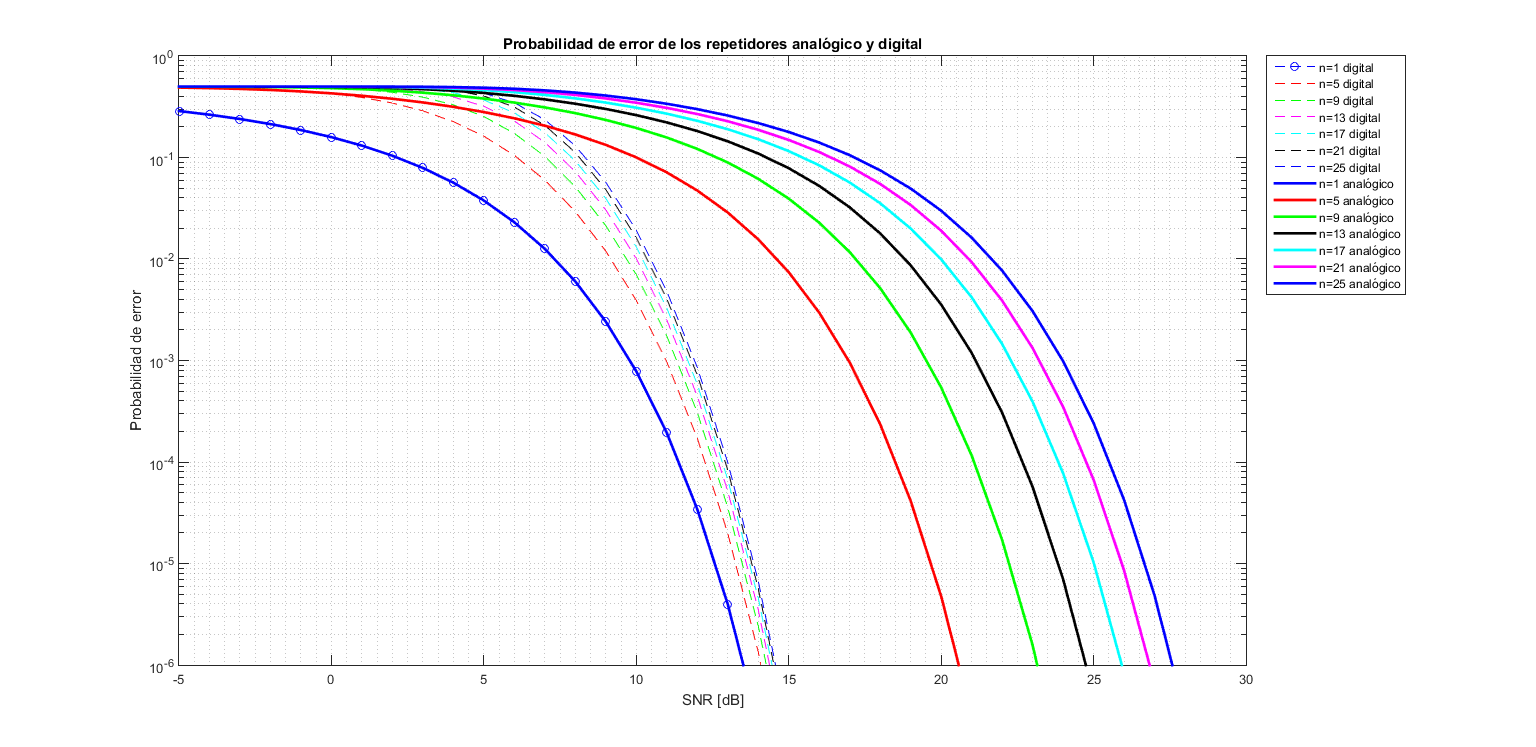
\includegraphics[width=1\textwidth]{images/Pe_pto3_1}
  \caption{Probabilidad de error de ambos sistemas con diferentes parámetros de SNR y número de etapas (n).}
  \label{fig:pto3_1}
\end{figure}

\hfill

De la figura \ref{fig:pto3_1} vemos que para cada $n$ ambos sistemas coinciden en un valor de SNR, los valores son los siguientes:

\begin{itemize}
\item 5 a -0.4 dB.
\item 9 a 0.4 dB.
\item 13 a 0.6 dB.
\item 17 a 1 dB.
\item 21 a 1.1 dB.
\item 25 a 1.2 dB.
\end{itemize}

Para cualquier número $n$ de etapas se repite el mismo comportamiento. Hasta la igualdad, ambos sistemas tienen una relación $SNR-P_e$ similar (casi idénticas). Luego de la misma, el sistema digital tiene una disminución significativamente más rápida con el aumento de la SNR.\\

Por lo tanto, conociendo el rango de SNR con el que se va a trabajar, la mejor opción es el sistema digital respecto de la Probabilidad de error en un amplio rango de valores.\\
Si el dato con el que se cuenta es la cantidad de etapas $n$, nuevamente el sistema digital es el más eficiente. En ambos casos cuando se supere ese ``umbral'' en el que ambos sistemas se comportan de manera similar.




\textbf{Ejercicio 4.}

\textbf{4.1}. Simulación de Montecarlo.

Realizamos una simulación sobre los valores de SNR dentro del intervalo  [5, 25] en dB.

Por cada valor del SNR se simularon N = 20000 veces para obtener un resultado ``óptimo´´, o sea, que los resultados concuerden con los cálculos teóricos. Los que se pueden ver claramente en las figuras \ref{fig:pto4_1} y \ref{fig:pto4_2}

\begin{figure}[H]
  \centering
  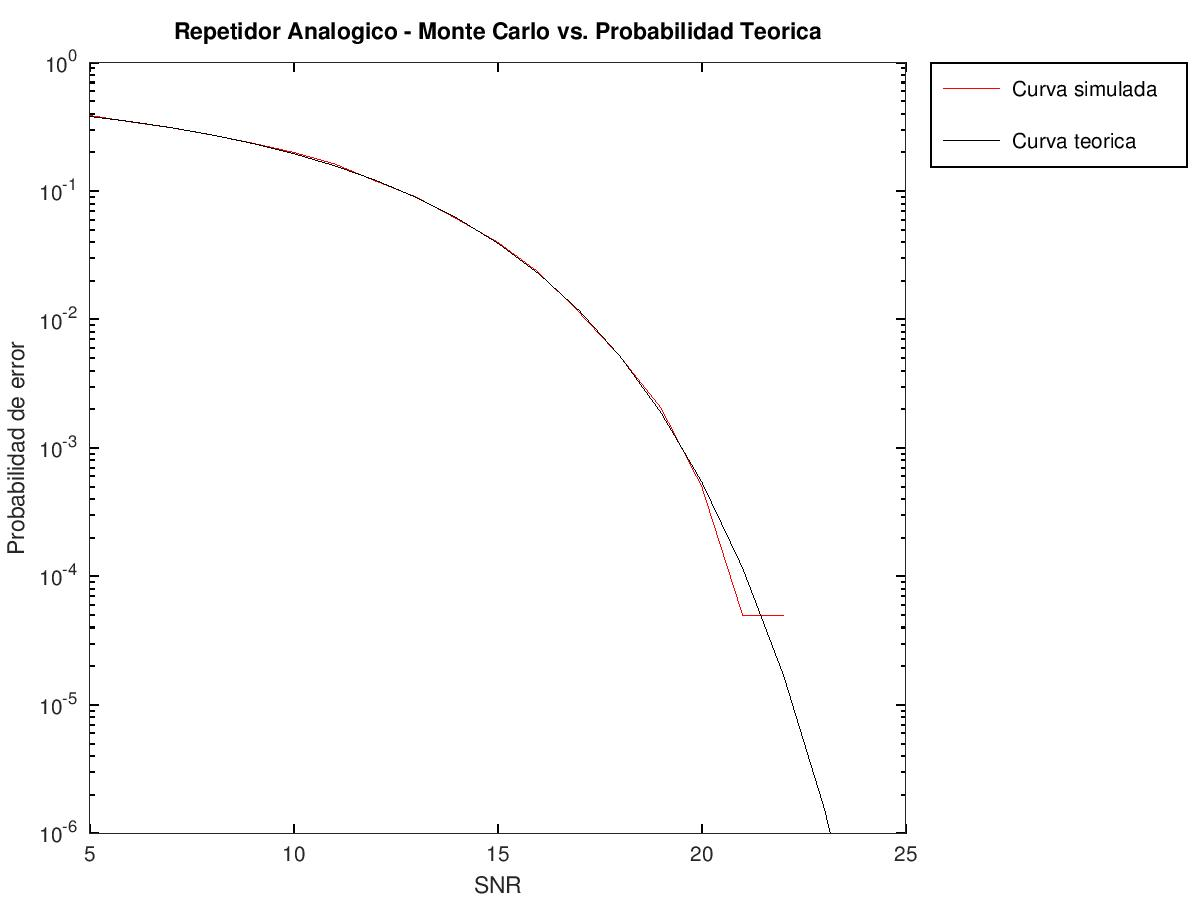
\includegraphics[width=1\textwidth]{images/Pe_pto4_1}
  \caption{Simulación de MonteCarlo para etapa analógica.}
  \label{fig:pto4_1}
\end{figure}

\begin{figure}[H]
  \centering
  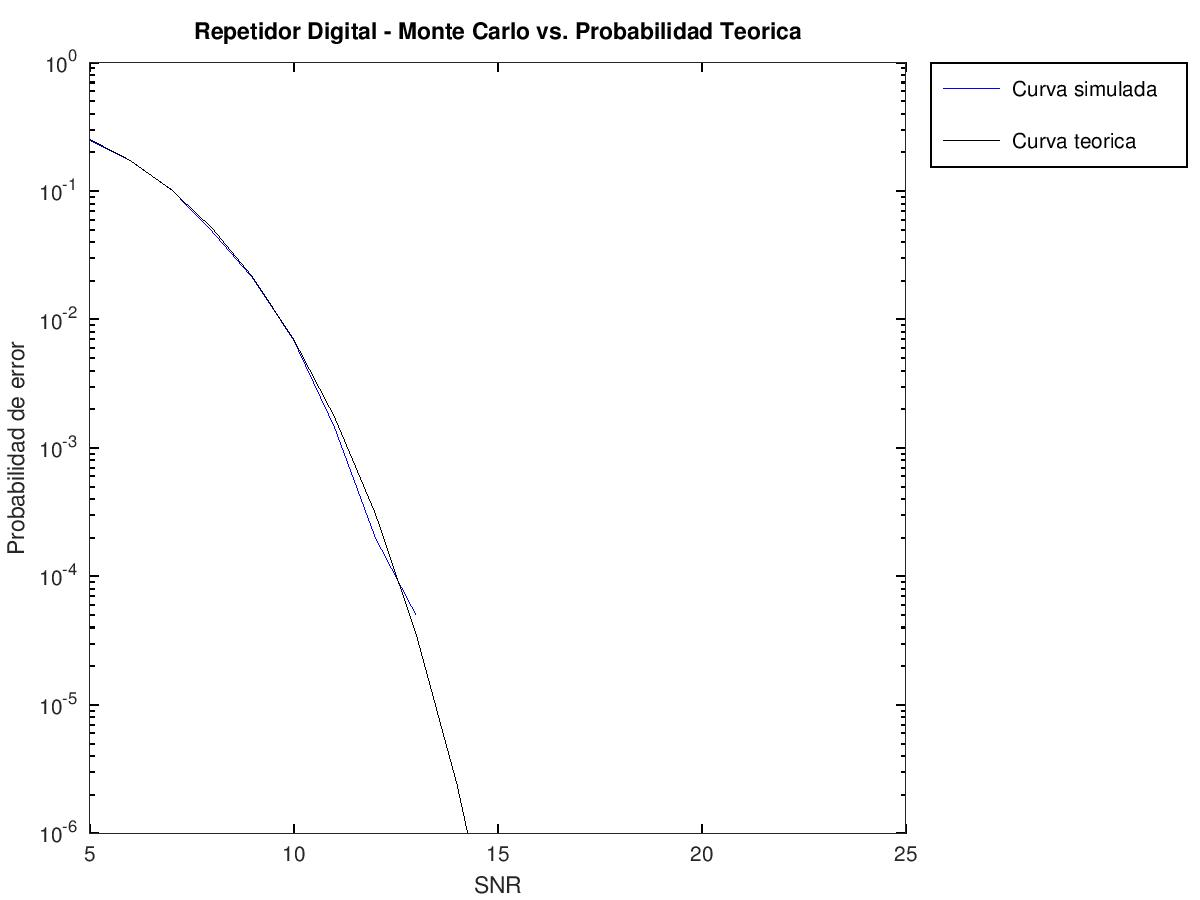
\includegraphics[width=1\textwidth]{images/Pe_pto4_2}
  \caption{Simulación de MonteCarlo para etapa digital.}
  \label{fig:pto4_2}
\end{figure}


\textbf{4.2}. Curvas de probabilidad.

Por un lado se simuló el circuito y por otro lado se propuso un modelo porbabilistico a priori que suponemos va a ajustar a nuestro circuito.
Por medio del resultado se verifica, al ver que las curvas son tan próximas, que el modelo propuesto es válido para representar el modelo real.
Se ve claramente que las curvas que se obtuvieron en la simulación se aproximan a las teóricas calculadas anteriormente. Esto se debe a que se hicieron las simulaciones ``correctamente''. Las realizaciones son efectivamente independientes. 

\newpage
%Los resultados confirman al encontrarse tan cercanos unos del otro lo calculado en la parte teórica, debido a la gran cantidad de simulaciones.

\textbf{4.3} Densidades de probabilidad de $Y_n$ (justo antes del detector) en el sistema analógico.

\begin{figure}[H]
  \centering
  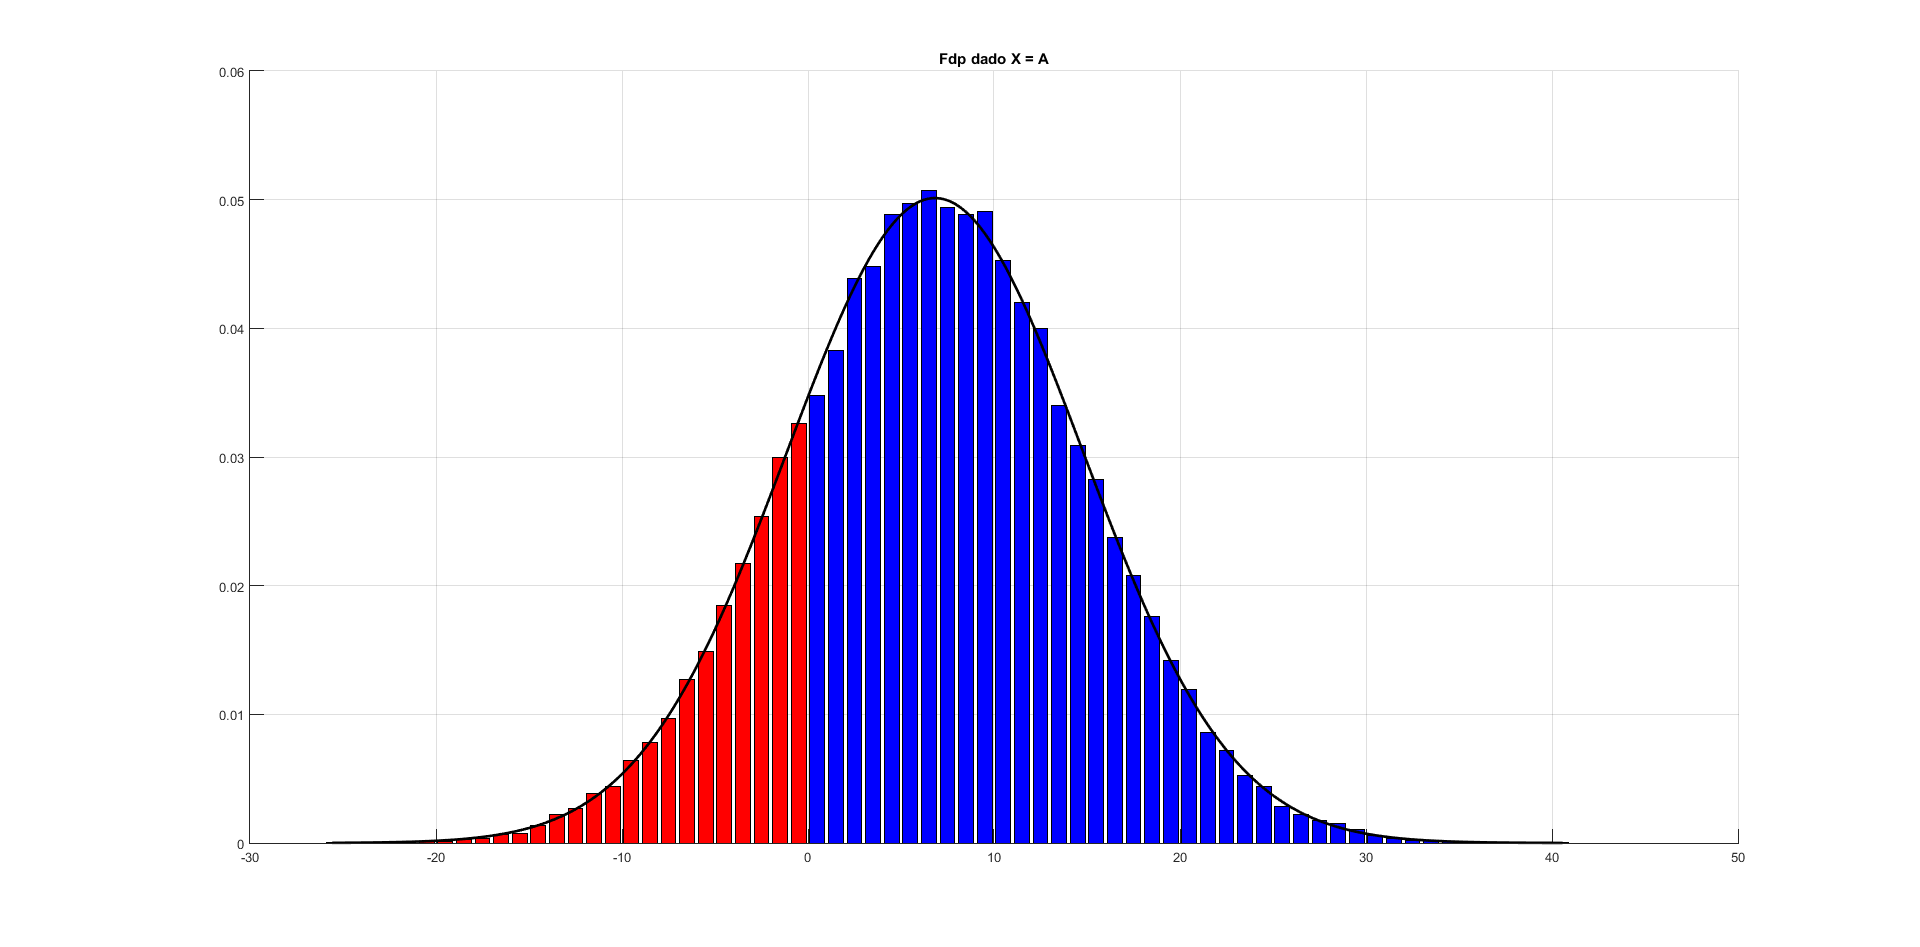
\includegraphics[width=1\textwidth]{images/fdp_XA}
  \caption{Función de densidad de probabilidad $f_{Y_n|X=A}$. En rojo los eventos de Error.}
  \label{fig:pto4_3}
\end{figure}	

\begin{figure}[H]
  \centering
  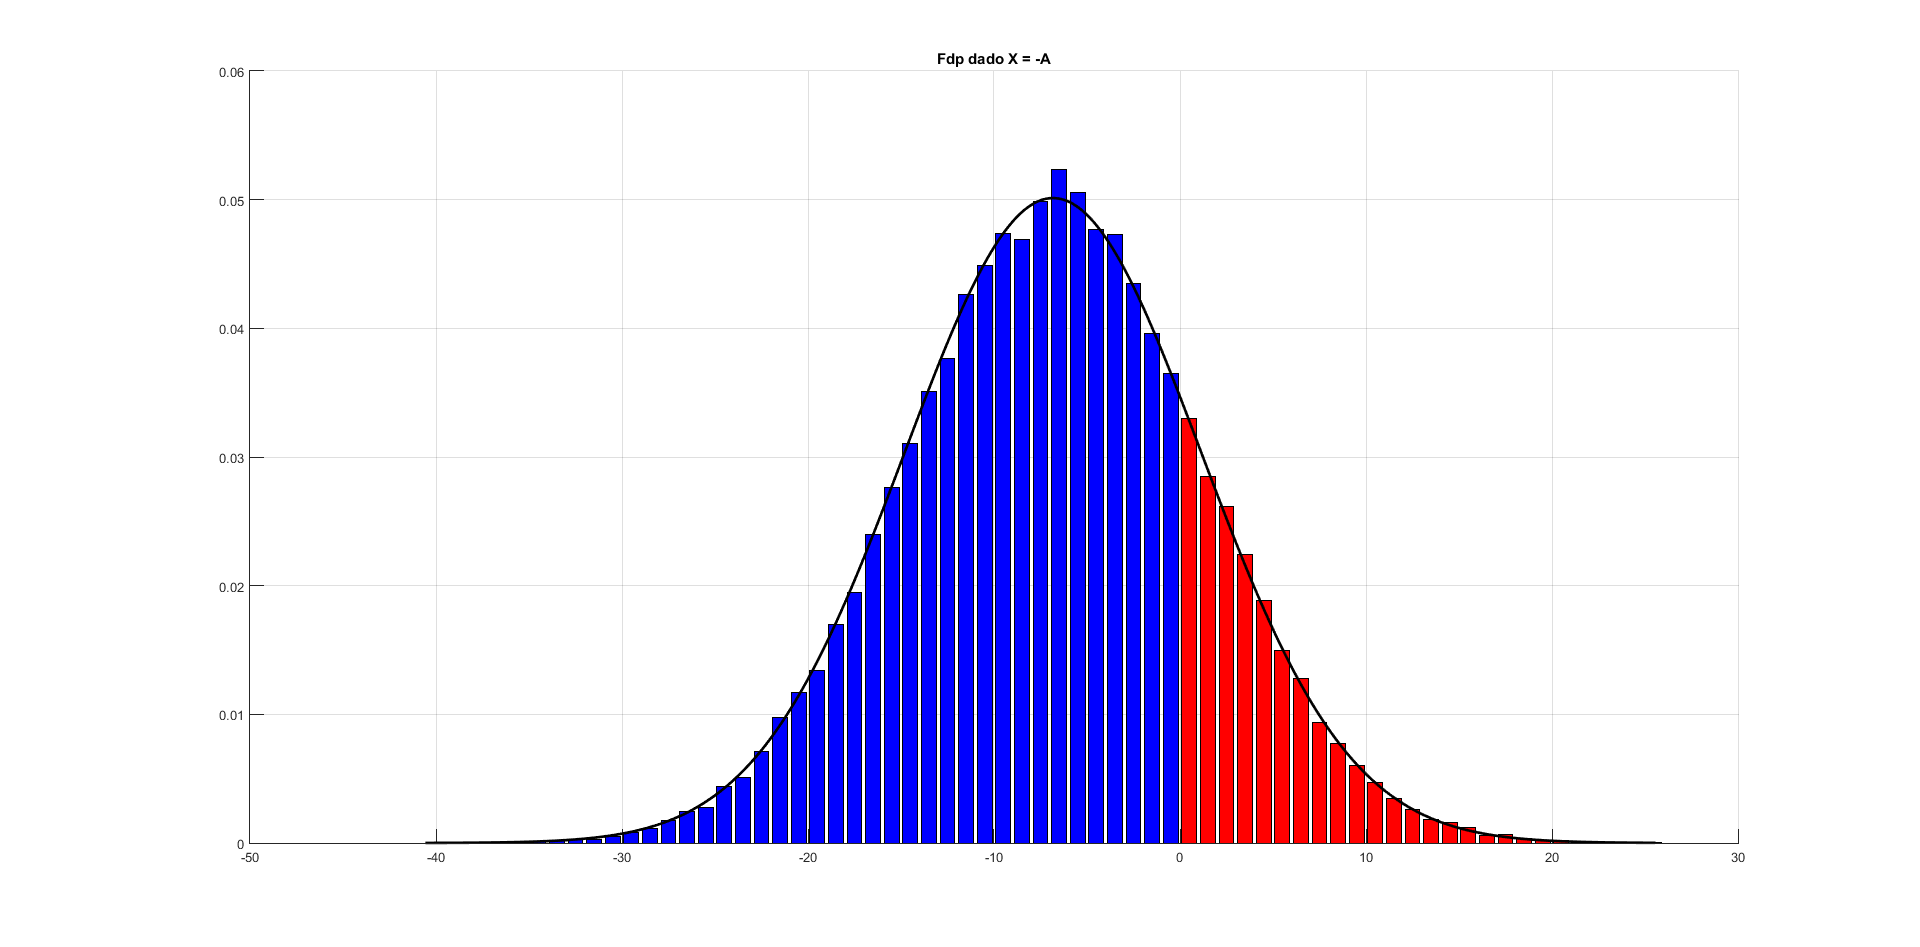
\includegraphics[width=1\textwidth]{images/fdp_X-A}
  \caption{Función de densidad de probabilidad $f_{Y_n|X=-A}$. En rojo los eventos de Error.}
  \label{fig:pto4_3b}
\end{figure}























